\begin{figure}
    \centering{
        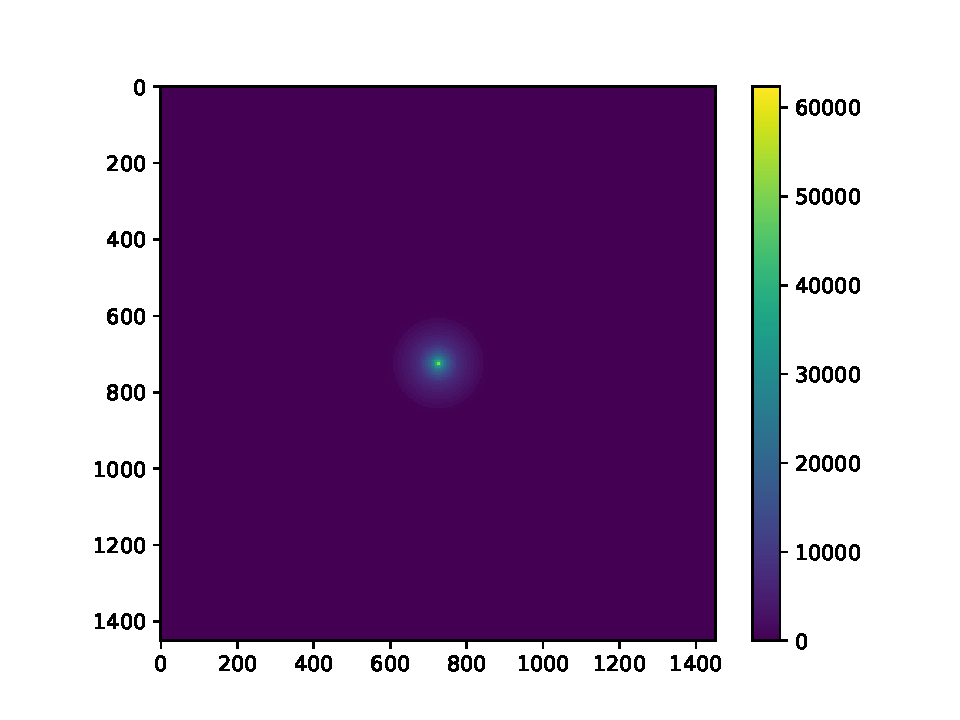
\includegraphics[scale=0.33]{figures/glory_duck/hawc/GD_mass_profiles/BootesI_plot.pdf}
        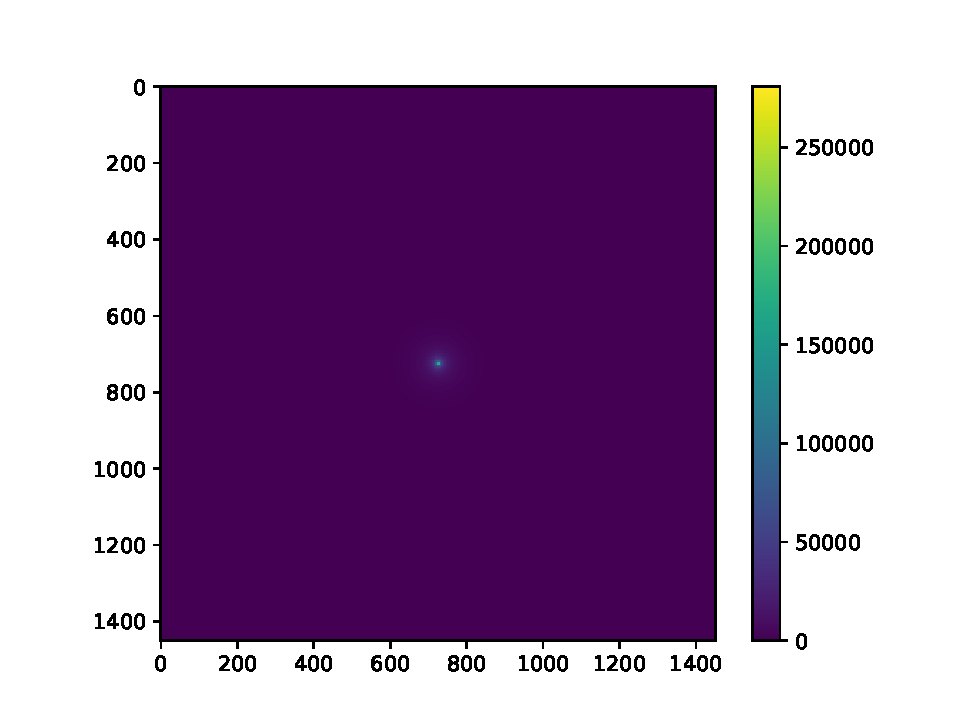
\includegraphics[scale=0.33]{figures/glory_duck/hawc/GD_mass_profiles/CanesVenaticiI_plot.pdf}
        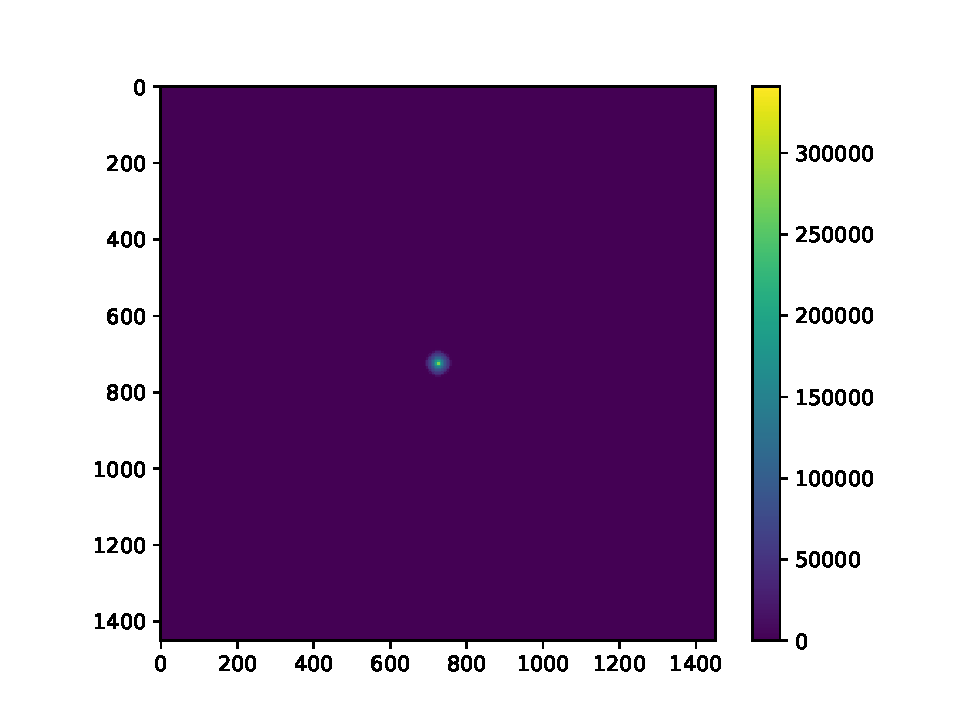
\includegraphics[scale=0.33]{figures/glory_duck/hawc/GD_mass_profiles/CanesVenaticiII_plot.pdf}
        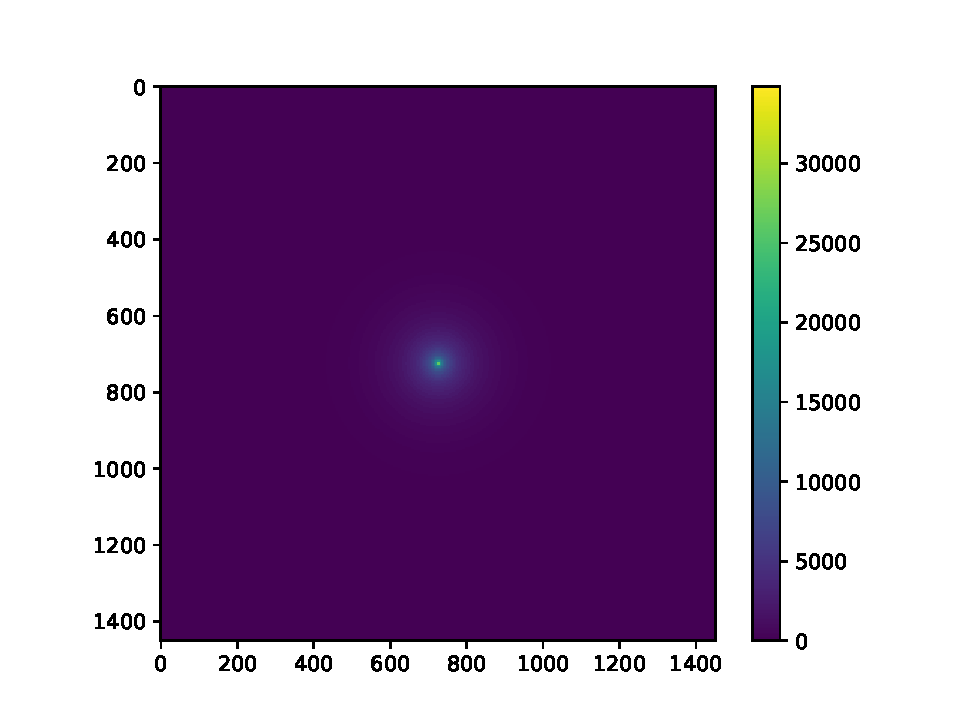
\includegraphics[scale=0.33]{figures/glory_duck/hawc/GD_mass_profiles/Draco_plot.pdf}
        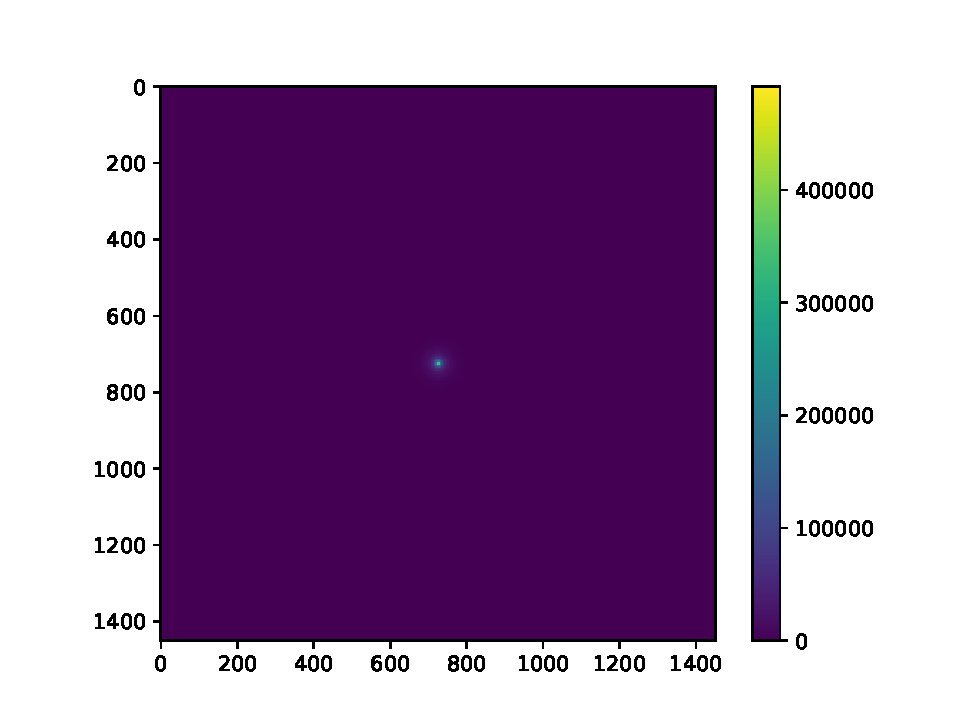
\includegraphics[scale=0.33]{figures/glory_duck/hawc/GD_mass_profiles/Hercules_plot.pdf}
        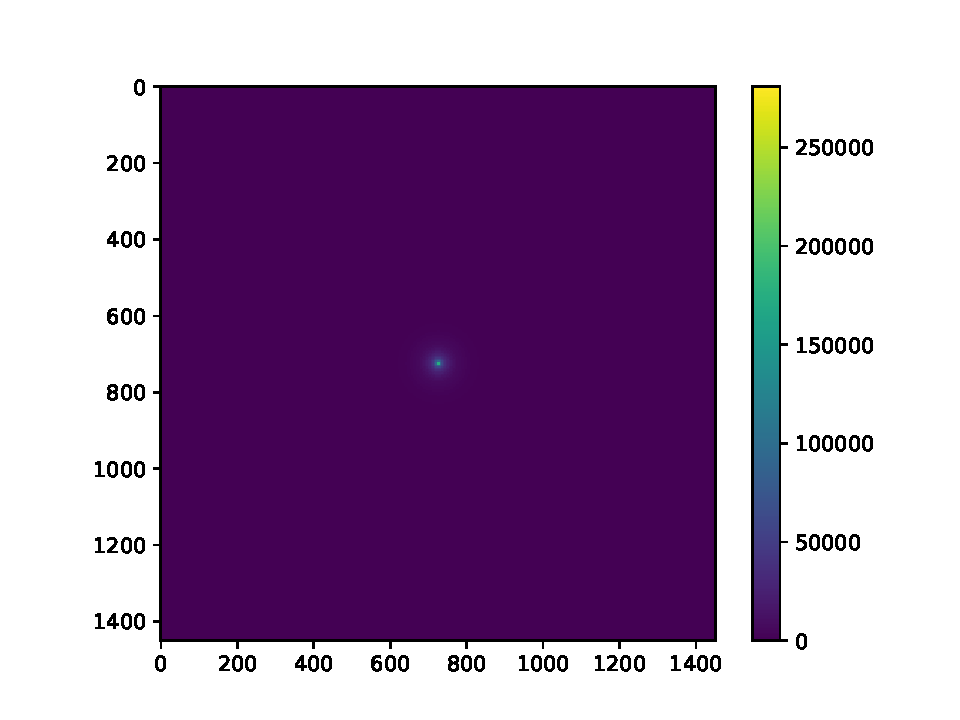
\includegraphics[scale=0.33]{figures/glory_duck/hawc/GD_mass_profiles/LeoI_plot.pdf}
        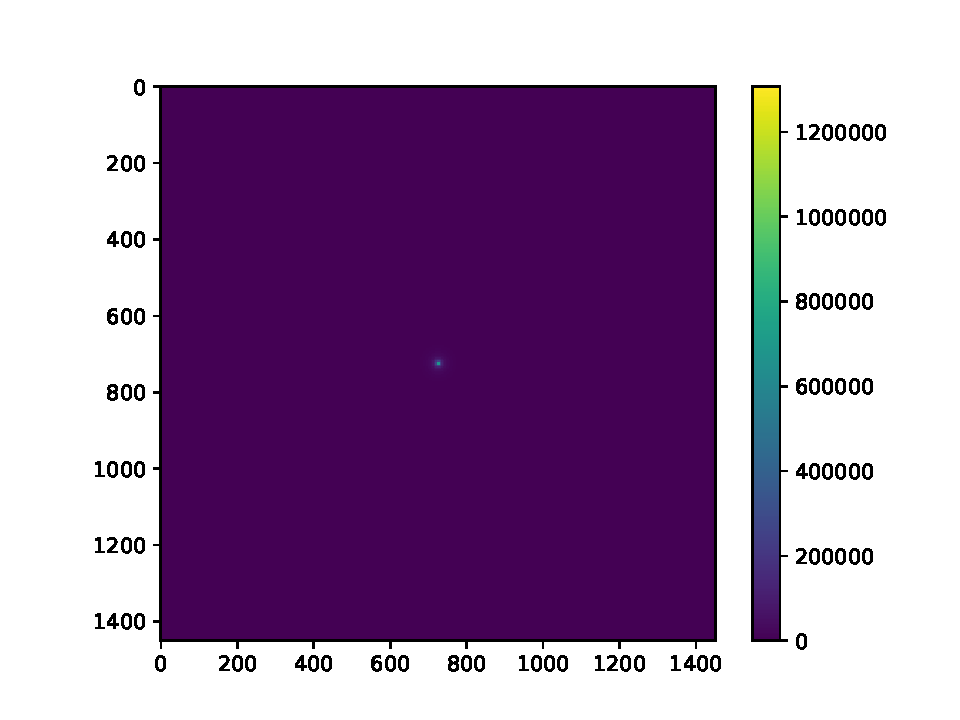
\includegraphics[scale=0.33]{figures/glory_duck/hawc/GD_mass_profiles/LeoII_plot.pdf}
        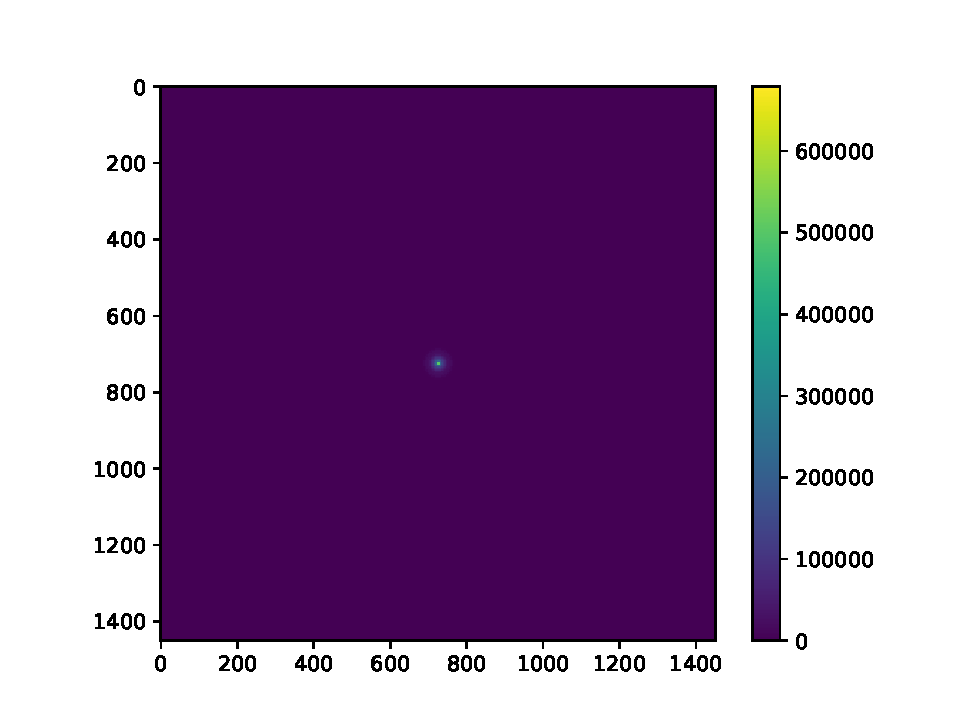
\includegraphics[scale=0.33]{figures/glory_duck/hawc/GD_mass_profiles/LeoIV_plot.pdf}
        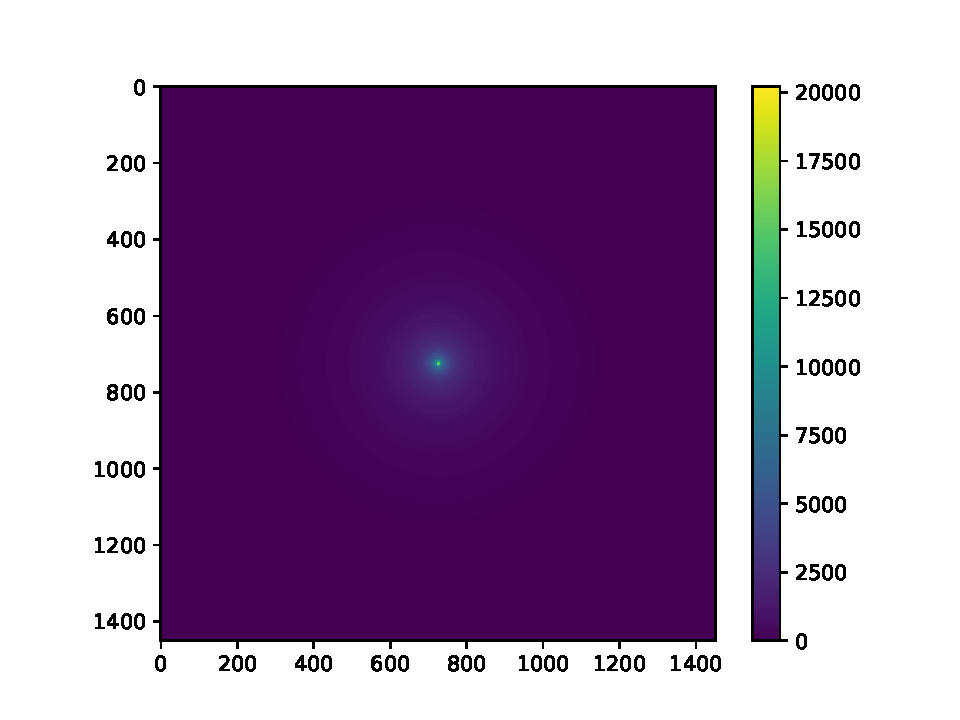
\includegraphics[scale=0.33]{figures/glory_duck/hawc/GD_mass_profiles/Sextans_plot.pdf}
        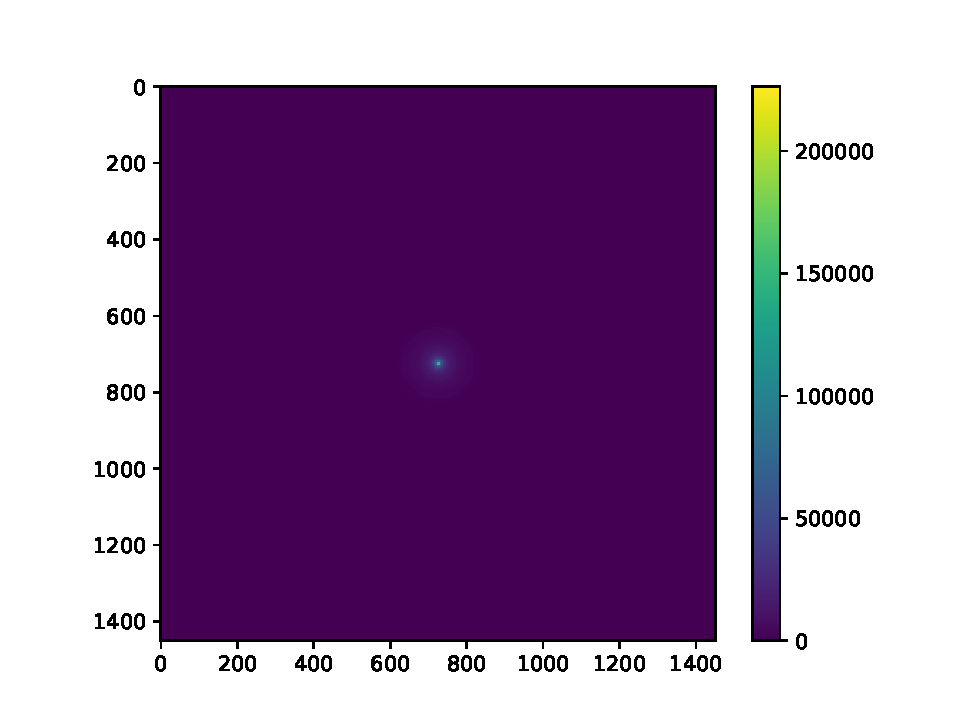
\includegraphics[scale=0.33]{figures/glory_duck/hawc/GD_mass_profiles/UrsaMajorI_plot.pdf}
        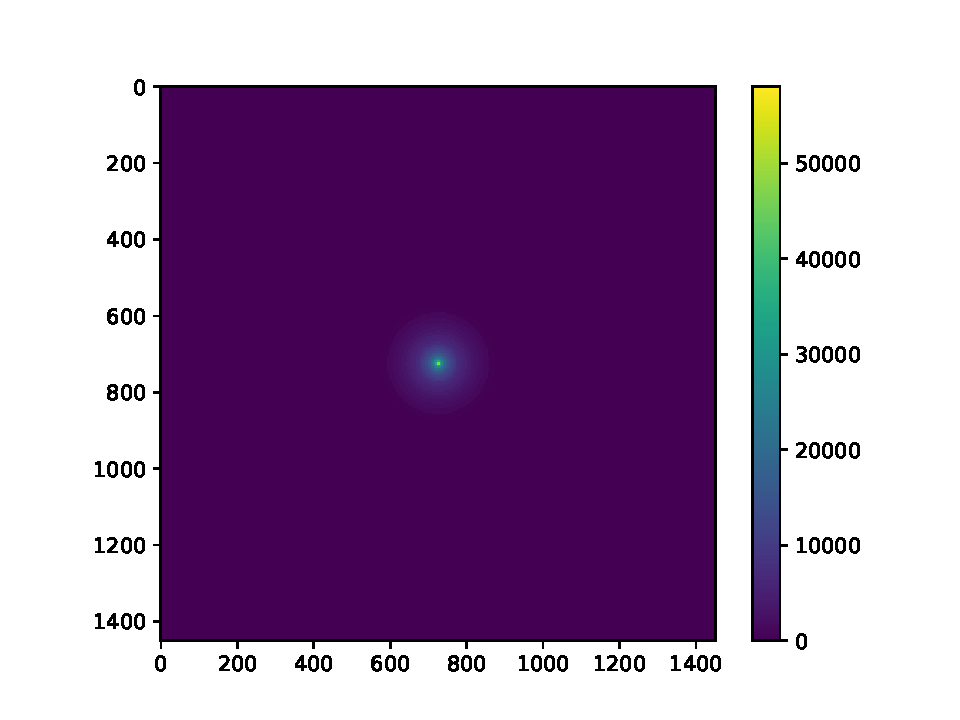
\includegraphics[scale=0.33]{figures/glory_duck/hawc/GD_mass_profiles/UrsaMajorII_plot.pdf}
    }
    \caption{Sister figure to \Cref{fig:gd_spatialmodel}. Sources in the first row from left to right: Bootes I, Canes Venatici I, II. In second row: Draco, Hercules, Leo I. In the first row: Leo II, Leo IV, Sextans. In the final row: Ursa Major I, Ursa Major II.} \label{fig:apx_gd_spatialmodels}
\end{figure}